\section{Experiments}
\label{sec:experiments}
A series of experiments were conducted to evaluate the performance of
classical and quantum transformer models using different encoding
techniques and variations of quantum circuit-based layers. The goal
was to compare these models not only in terms of
their accuracy but also in their training speed across different
computational setups. To avoid inconsistencies in the implementation,
we also refactored and aligned the model frameworks for fair comparison.

The experiments were performed on three datasets: IMDb, Amazon, and
Yelp, each preprocessed and tokenised with a maximum sequence length
of 128 tokens. The IMDb dataset was used for models both with and
without embedding layers, while the Amazon and Yelp datasets were
only used for models without embedding layers. A sampling strategy
was applied to ensure the appropriate dataset size for training.

Two broad categories of models were tested. The first category
involved models with embedding layers, where the vocabulary size was
set to 50,000, and the architecture included two transformer layers,
each with two multi-head attention heads. Quantum models in this
category employed angle encoding using either \(R_x\) or \(R_z\) gates,
integrated with either basic or strong \glspl{VQC}, where the number
of quantum layers varied between 3 and 8.
For certain models, amplitude encoding was also explored using
TensorFlow-CPU as the backend for TensorCircuit.

For models without embedding layers, we used external \gls{BERT} embeddings
with fixed embedding sizes of 8 and 256 dimensions. These models were
tested in both classical and quantum variants, applying either angle
or amplitude encoding. The quantum circuits used in these experiments
involved both basic \gls{VQC} architectures, with a single layer of
parameterised gates followed by CNOT gates, and strong \gls{VQC}
architectures, with three layers of parameterised gates. Across all
models, the training process was handled with the same set of
hyperparameters, ensuring consistent learning conditions for each experiment.

Due to the fact that TensorCircuit only supports \gls{JIT} compilation and
vectorised parallelism on TensorFlow and not PyTorch, we initially
created what might be termed a "Frankenstein" model—combining a
classical model implemented in PyTorch with a quantum model in
TensorCircuit (which uses TensorFlow). To address this inconsistency
across frameworks, we developed a new version of the transformer
model in TensorFlow. This unified approach allows both classical and
quantum models to share the same backend, ensuring compatibility in
CUDA versions. Due to CUDA version conflicts, the TensorFlow setup
was initially limited to CPU. However, the new model in TensorFlow
was designed specifically to utilise TensorFlow CUDA for
TensorCircuit. This enabled a comparison of training speed between
CPU and CUDA-enabled systems. The newly created models were
refactored and tested against their older counterparts to measure
improvements in training speed.

The following models were tested for training time:

\begin{enumerate}
  \item The original PyTorch-based quantum model using GPU with PennyLane.
  \item The original PyTorch-based quantum model using CPU with PennyLane.
  \item The refactored PyTorch-based quantum model using GPU with PennyLane.
  \item The refactored PyTorch-based quantum model using CPU with PennyLane.
  \item The original PyTorch-based quantum model using TensorCircuit with
    TensorFlow-CPU as the backend.
  \item The refactored PyTorch-based quantum model using TensorCircuit
    with TensorFlow-CPU as the backend.
  \item The refactored TensorFlow-based quantum model using TensorCircuit
    with TensorFlow-CUDA as the backend.
\end{enumerate}

Each of these models was trained for 4 epochs, and the average
training time across these epochs was recorded for comparison. This
allowed us to evaluate any potential speed increases when switching
to a TensorFlow-CUDA backend for TensorCircuit, and whether the
refactored models offered performance improvements over the original
implementations.

The hyperparameters across all experiments were consistent. The
learning rate was set at 0.001, with the Adam optimiser applied
across both classical and quantum models. For most experiments, a
batch size of 64 was used. A maximum sequence length of 128 was
enforced for all input data, and each model utilised two multi-head
attention layers and two transformer layers. The StepLR learning rate
scheduler, with a step size of 5 and gamma of 0.1, was used for
dynamic learning rate adjustment. For all models, the loss function
was Binary Cross-Entropy with Logits Loss (BCEWithLogitsLoss), which
combines the sigmoid activation and binary cross-entropy into a
single step. The model outputs logits (raw scores), which are passed
through a sigmoid function to transform them into probabilities
between 0 and 1. These probabilities are then used to compute the
binary cross-entropy loss, measuring how well the predicted
probabilities match the true binary labels.

\section{Results and Analysis}
\label{sec:results_analysis}
Our experimental results comparing classical and quantum transformer
models with different encoding strategies are presented and analysed
below. The experiments were conducted over various datasets, both
with and without embedding layers, and across multiple quantum circuit designs.

\subsection{Transformers with Embedding Layers}
\label{subsec:transformers_with_embedding_layers}
The experiments on models with embedding layers focused on comparing
classical transformer models with quantum models that utilised angle
encoding encoding integrated with basic and strong \glspl{VQC}
parameterised by the \(R_x\) gate. The
dataset sizes ranged from 3,200 to 5,000, and the models were trained
for 30 epochs.

\begin{figure}[h]
  \begin{center}
    \subfloat[Classical vs. Quantum Model with Angle Encoding (Basic
    \gls{VQC})]{
      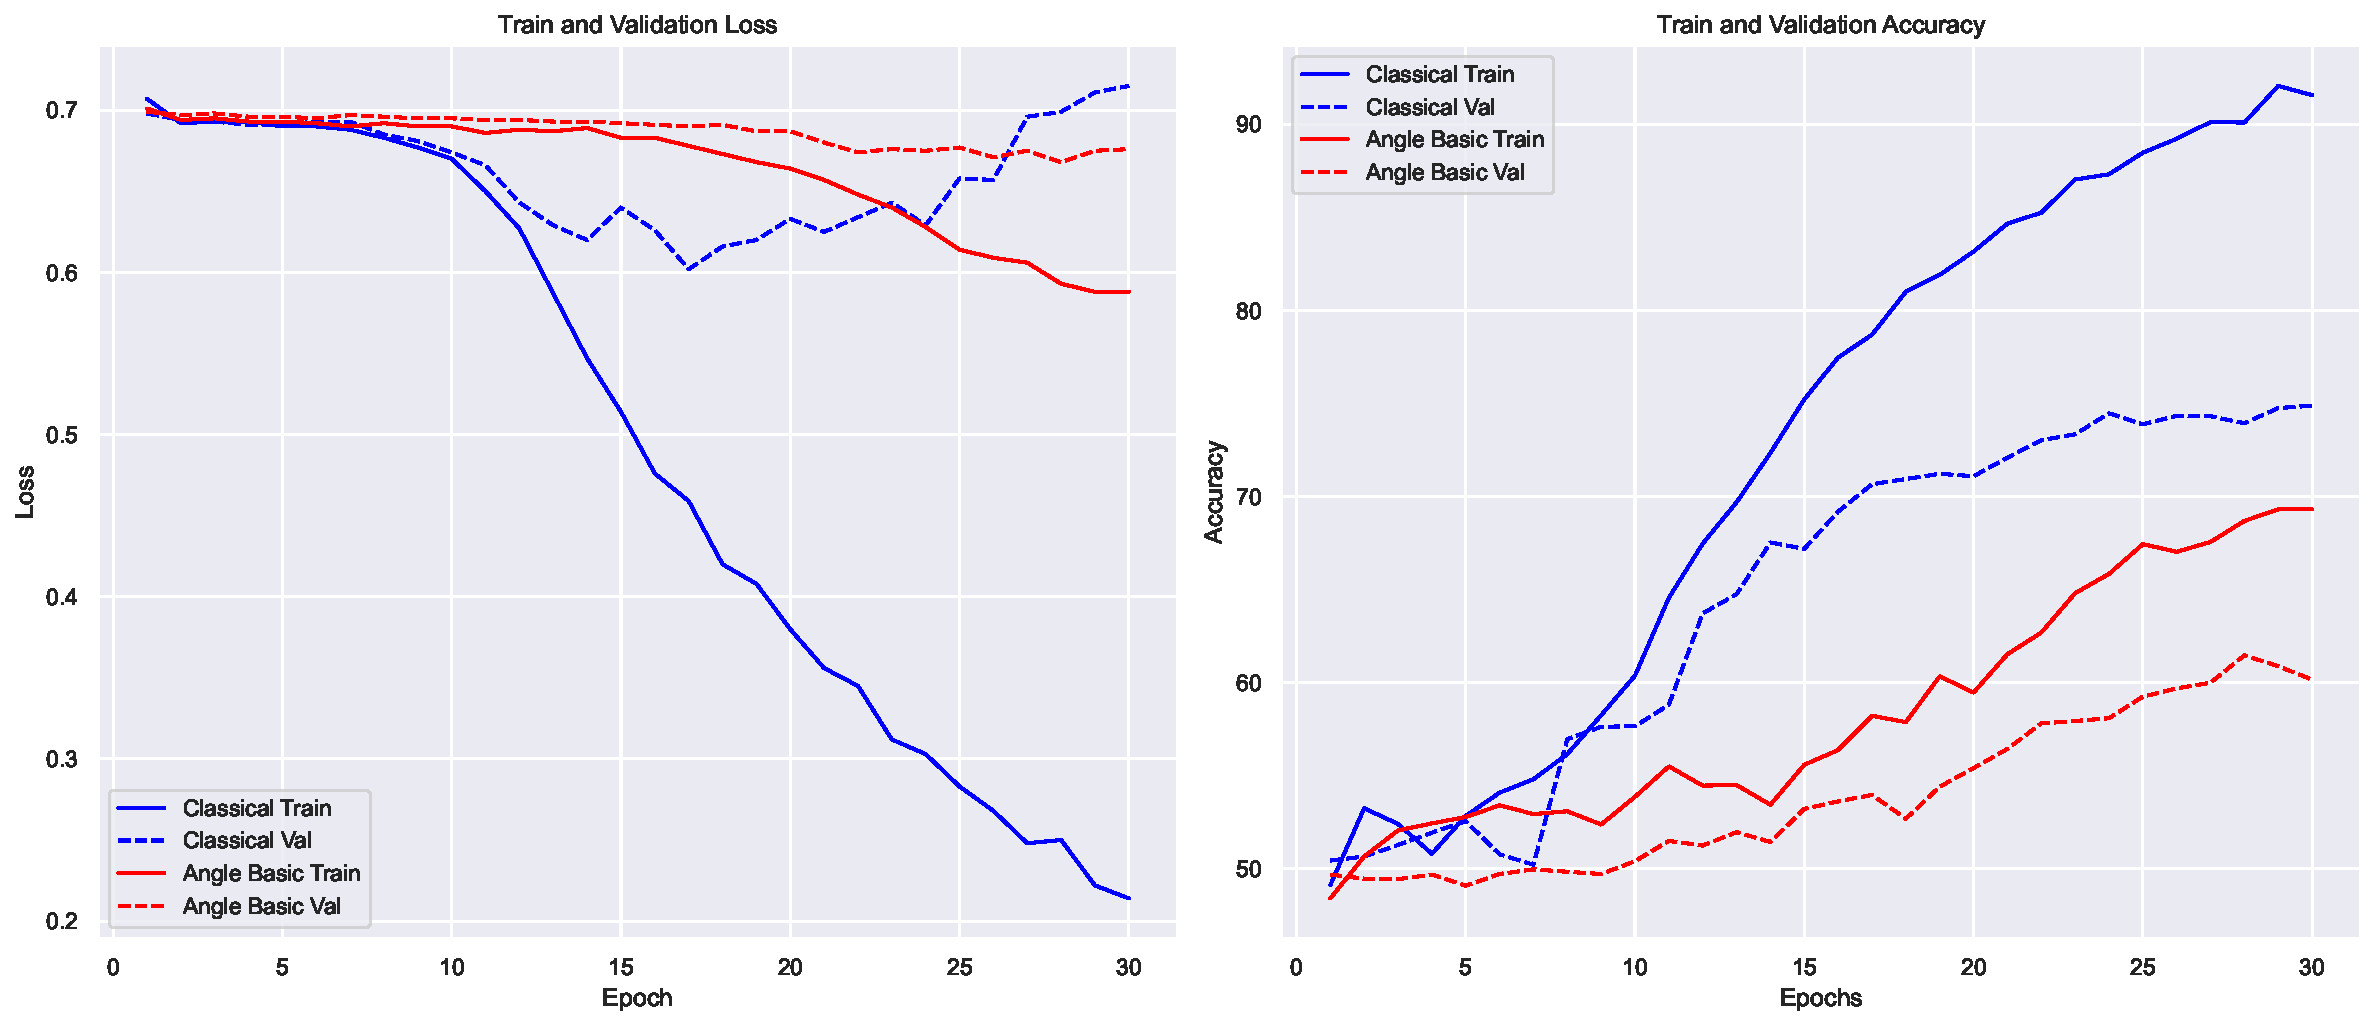
\includegraphics[width=0.98\textwidth]{img/plots/0_1.pdf}
    }
  \end{center}
  \vspace{-0.5cm}
  \caption{A loss plot and an accuracy plot for the classical and
    quantum models on the IMDb dataset (3,200 samples), with 50,000
    vocab size and 64 batch size, trained for 30 epochs. The plot
    compares the classical transformer model with a quantum transformer
  using angle encoding and 8 layers of basic \glspl{VQC}.}
  \label{fig:0_1}
\end{figure}

The loss plot in \autoref{fig:0_1} shows the performance of two models: a
classical transformer (blue) and a quantum model (red) with 8 layers
of VQCs. For
the classical model, overfitting is evident, as the training loss
continues to decrease while the validation loss starts to diverge
after the 17th epoch. At the lowest point, the validation loss
reaches approximately 0.6 at the 17th epoch, while the training loss
is around 0.42. These relatively high loss values indicate that the
model is not performing optimally. In contrast, the quantum model
shows little improvement in loss reduction until the 15th epoch,
after which it starts to decrease slowly. By the 20th epoch, the
quantum model's training loss is 0.66, and its validation loss is
0.69, indicating that the quantum model struggled to learn
effectively as both models began with a loss value of 0.7.

The accuracy plot in \autoref{fig:0_1} further highlights the
classical model's superior
performance. The classical model achieves a peak validation accuracy
of 0.75, while the quantum model's validation accuracy only reaches
0.61. Additionally, there is a noticeable gap between the training
and validation accuracy for the classical model, further confirming
the presence of overfitting.

While the quantum model begins to learn around the 15th epoch, we
stopped training at the 30th epoch. This suggests that extending the
training could potentially allow the quantum model to learn further.
However, this experiment was preliminary, designed to evaluate
whether the quantum model could be trained within a feasible amount
of time. Moving forward, further optimisations are necessary to
enhance its learning efficiency and accuracy.

The poor performance of both models in terms of loss and accuracy can
largely be attributed to the limited size of the dataset used and the
challenges faced by the quantum model due to the depth of its
circuit. For future experiments, increasing the dataset size and
reducing the circuit depth could potentially yield better results and
allow the quantum model to learn faster and more effectively.

\begin{figure}[h]
  \begin{center}
    \subfloat[Classical vs. Quantum Models with Different Quantum
    Configurations]{
      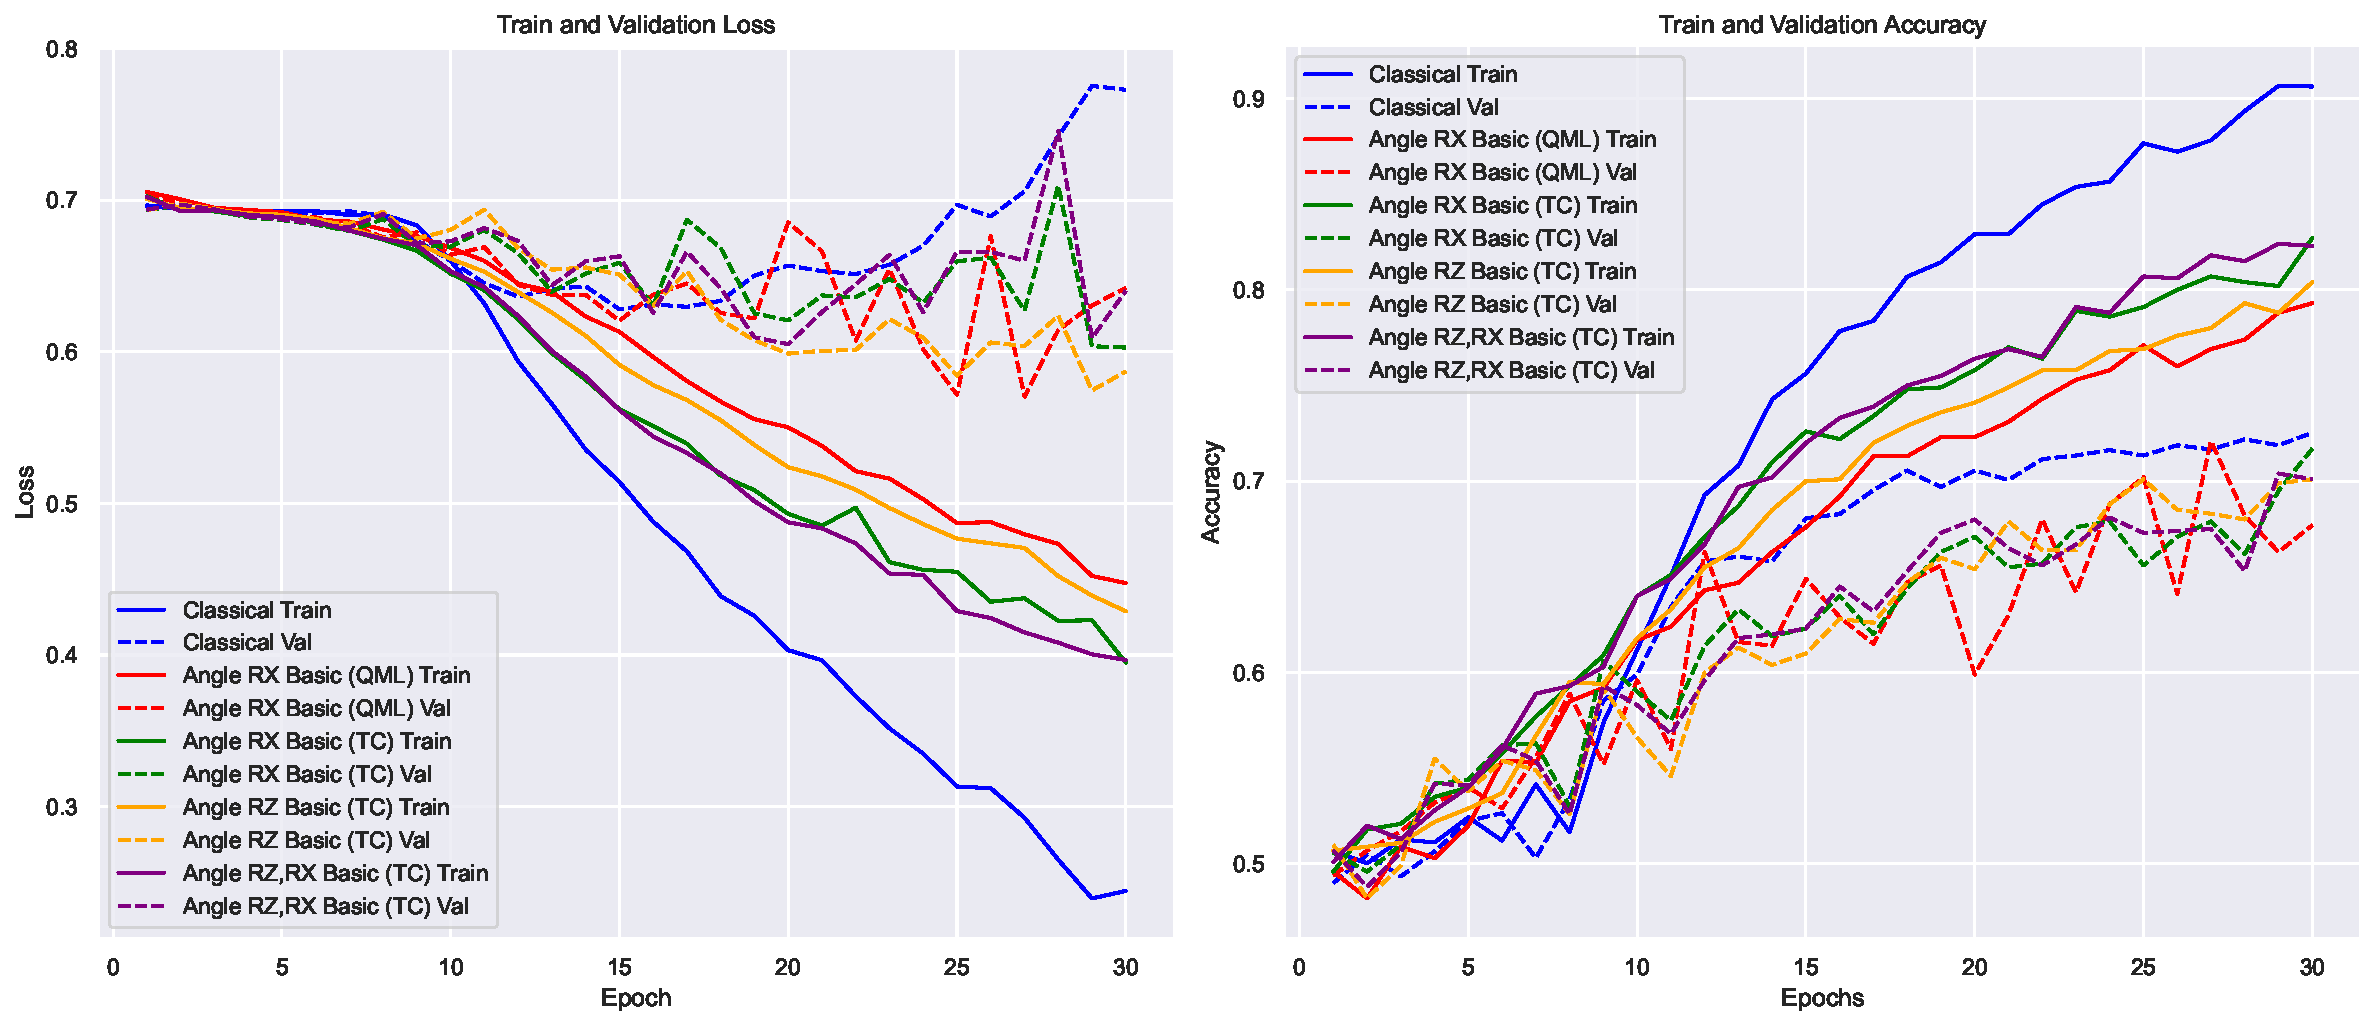
\includegraphics[width=0.98\textwidth]{img/plots/2_3_4_5_6.pdf}
    }
  \end{center}
  \vspace{-0.5cm}
  \caption{A loss plot and an accuracy plot for classical and quantum
    models on the IMDb dataset (5,000 samples), with a vocab size of
    50,000 and a batch size of 32, trained over 30 epochs. The figure
    compares the classical model with quantum models using various
    configurations of angle encoding (\(R_x\) and \(R_z\) gates) and backends
  (QML and TensorCircuit) with 3 layers of \glspl{VQC}.}
  \label{fig:2_3_4_5_6}
\end{figure}

In this experiment, we increased the dataset size to 5,000 samples
and tested four quantum models with different configurations. To
explore potential performance improvements, we reduced the batch
size, hoping it would enhance the ability of the models to generalise and
achieve higher accuracy.

The loss plot in \autoref{fig:2_3_4_5_6} reveals that all models,
including the classical and
quantum models, exhibit overfitting. While the training losses for
all quantum models closely follow the training
loss of the classical model (blue), the validation losses remain
problematic. None of the models
achieve a validation loss below 0.6, with all models starting at
approximately 0.7. The fluctuation observed in the validation loss,
particularly for the quantum models, indicates instability during
training, suggesting that the batch size may be too small for stable
generalisation.

When examining the accuracy plot in \autoref{fig:2_3_4_5_6}, it is
clear that the classical
model still outperforms all quantum models. Among the quantum models,
the configuration with two layers of angle encoding (purple) shows marginally
better performance during training but results in similar validation
accuracies to the other quantum models. This suggests that varying
the rotation gate or adding additional layers of angle encoding does
not significantly improve performance. The substantial fluctuations
in the validation accuracy of the quantum models further point to the
small batch size as a limiting factor in achieving stable training.

Given these results, future experiments should focus on extracting
the embedding layer and using a pre-trained model to encode the
documents. This approach may provide a stronger feature
representation and lead to improved accuracy. Additionally,
increasing the batch size back to 64 should help stabilise training
and improve the overall model performance, especially for the quantum
models. Finally, leveraging the full dataset could further refine the
learning capacity  of the quantum model learning capacity and boost
validation accuracy.

\subsection{Transformers without Embedding Layers}
\label{subsec:transformers_without_embedding_layers}
By eliminating the internal embedding layers, we aimed to assess how
well the models could handle these externally encoded inputs without
relying on the internal embedding layers. The models
were evaluated on the IMDb, Amazon, and Yelp datasets, using
embedding sizes of 8 for angle encoding and 256 for amplitude encoding,
with a batch size of 64 over 20 epochs.
The quantum models employed three layers of basic
and strong \glspl{VQC} parameterized by the \(R_z\) gate using 8 qubits.

\begin{figure}[h]
  \begin{center}
    \subfloat[IMDb Dataset - Classical vs. Quantum Models (Embedding
    Size 8 and 256)]{
      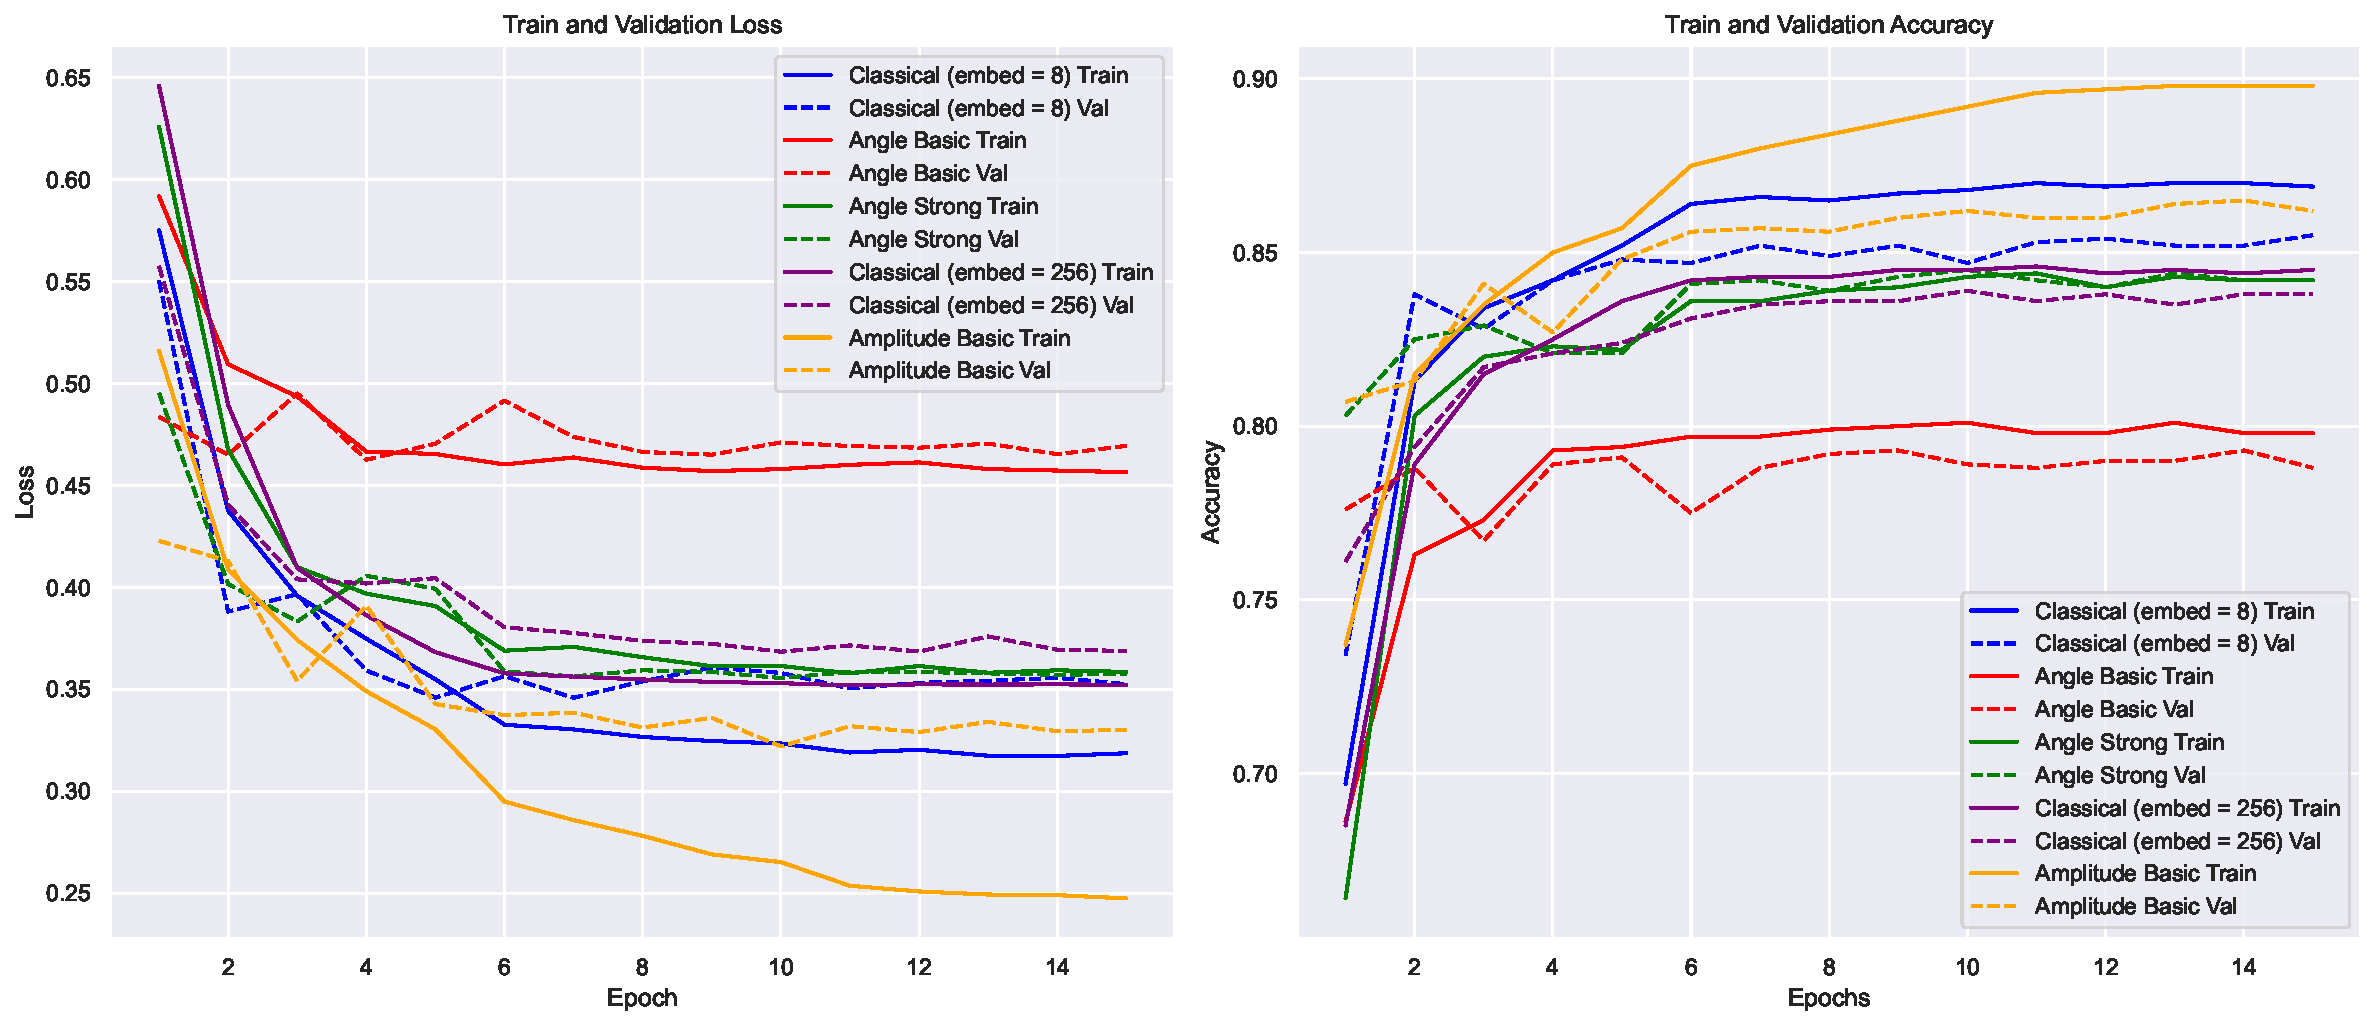
\includegraphics[width=0.98\textwidth]{img/plots/7_8_9_10_11.pdf}
    }
  \end{center}
  \vspace{-0.5cm}
  \caption{A loss plot and an accuracy plot for classical and quantum
    models on the IMDb dataset, using embedding sizes of 8 and 256,
    batch size of 64, trained over 20 epochs. The figures compare the
    classical transformer models to quantum models with angle encoding
    (3 layers of basic and strong \glspl{VQC}) and amplitude encoding
  (3 layers of basic \glspl{VQC}).}
  \label{fig:7_8_9_10_11}
\end{figure}

The loss plot in \autoref{fig:7_8_9_10_11} demonstrates that all
models are learning effectively, with no signs of overfitting or
instability. The absence of fluctuations in the validation loss
indicates that the batch size of 64 is well-suited for this
experiment. The loss values are generally low, signalling that the
models are optimising as expected. However, the quantum model using
angle encoding with a basic \gls{VQC} (red) is underperforming relative to
the other models, trailing by at least 0.1 in loss reduction. In
contrast, the quantum model with amplitude encoding and a basic \gls{VQC}
(yellow) is outperforming all other models, including the classical models.

Interestingly, the classical model with an embedding size of 8 also
performs better than the classical model with an embedding size of
256. This could suggest that smaller embedding sizes encourage the
model to learn more compact and efficient feature representations,
leading to improved performance. The quantum models with amplitude
encoding further highlight the effectiveness of this approach,
demonstrating that advanced quantum circuits may offer superior
learning capabilities in certain scenarios.

In the accuracy plot of \autoref{fig:7_8_9_10_11}, we observe similar
trends as seen in the loss plot. Even the worst-performing
model—again, the quantum model with angle encoding and a basic \gls{VQC}
(red)—achieves a solid accuracy of at least 0.78. Despite lagging
behind by approximately 0.08 compared to the other models, this still
represents a competitive performance. Moreover, the quantum model
with the strong \gls{VQC} (green) outperforms its counterpart with the
basic \gls{VQC}, indicating that increasing circuit complexity improves
accuracy, though not as drastically as one might expect.

The top-performing model is the quantum model using amplitude
encoding (yellow), which achieves an impressive accuracy of 0.86,
surpassing the classical models. This reinforces the notion that
amplitude encoding, when combined with quantum circuits, can provide
significant advantages in learning performance, especially when
compared to classical architectures and simpler quantum models.

In this study, one of our key objectives was to reproduce results
from prior research~\cite{Cherrat_2024}, which indicated that quantum
models have the
potential to outperform classical models. Based on these results, we
have successfully achieved this goal, with the quantum model using
amplitude encoding consistently outperforming the classical models in
both loss and accuracy. This confirms the findings from previous
studies and demonstrates that well-optimised quantum models can
indeed surpass classical models in certain learning tasks.

Overall, these models demonstrate substantial improvements over
previous configurations. The results indicate that quantum models,
particularly those using amplitude encoding, are capable of
outperforming classical models when tuned appropriately. Given the
promising results, the next logical step would be to test these
models on additional datasets to evaluate their generalisability and
robustness across different tasks. This would provide a more
comprehensive understanding of their strengths and limitations in
diverse scenarios.

\begin{figure}[h]
  \begin{center}
    \subfloat[Amazon Dataset - Classical vs. Quantum Models
    (Embedding Size 8 and 256)]{
      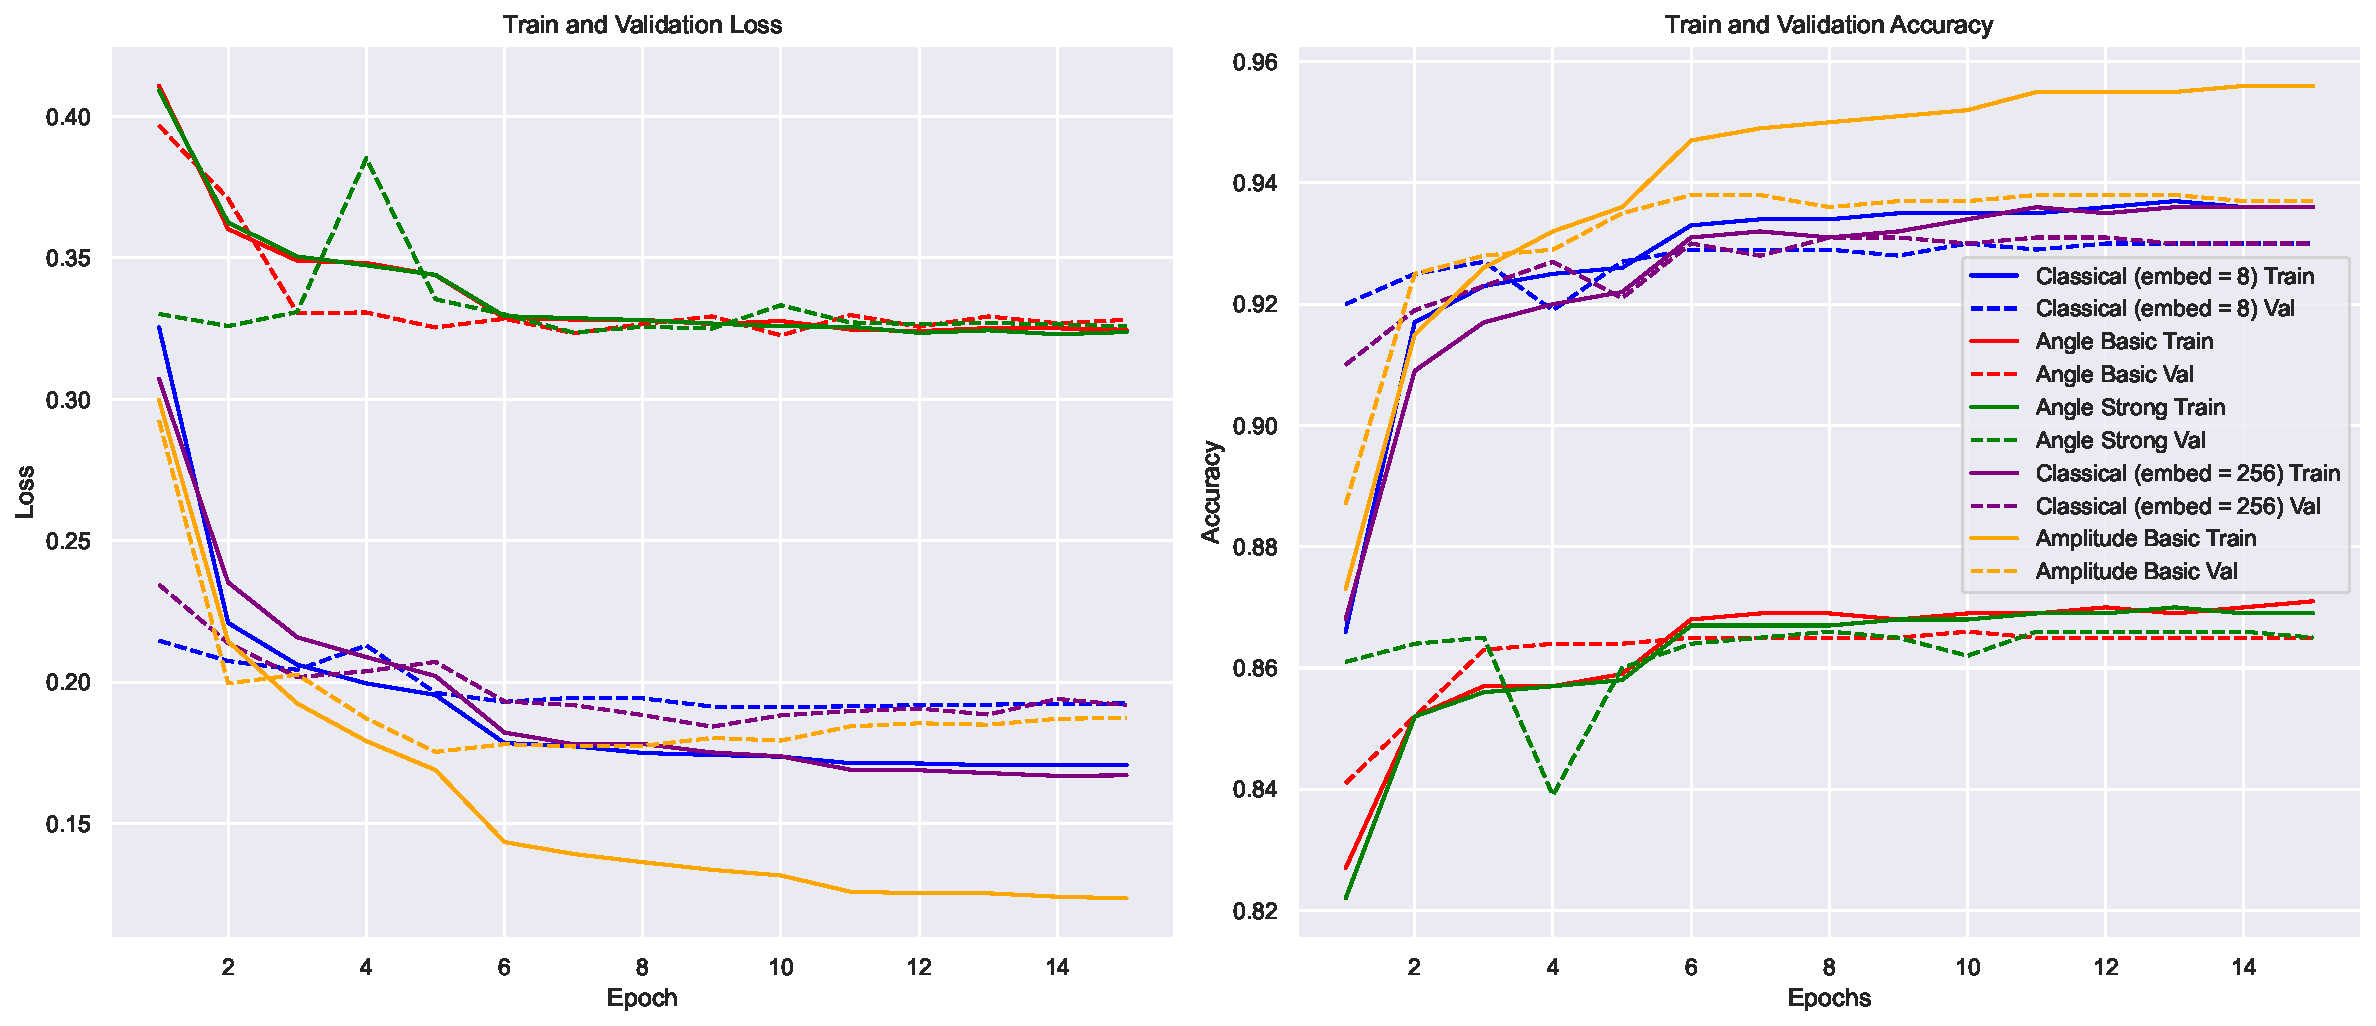
\includegraphics[width=0.98\textwidth]{img/plots/12_13_14_15_16.pdf}
    }
  \end{center}
  \vspace{-0.5cm}
  \caption{A loss plot and an accuracy plot for classical and quantum
    models on the Amazon dataset, with embedding sizes of 8 and 256,
    batch size of 64, trained for 20 epochs. The figures compare the
    classical transformer models to quantum models with angle encoding
    (3 layers of basic and strong \glspl{VQC}) and amplitude encoding
  (3 layers of basic \glspl{VQC}).}
  \label{fig:12_13_14_15_16}
\end{figure}

In the loss plot of \autoref{fig:12_13_14_15_16}, we can see that the
loss values across all models
appear to be optimally decreasing as training progresses. The
training losses consistently drop and eventually plateau, while the
validation losses show minimal decline, suggesting that the models
are generalising effectively. Interestingly, the quantum model using
a strong VQC (green), which previously performed better, now lags
behind both the classical models and the quantum model with amplitude
encoding. The strong VQC exhibits a notable spike around the 4th
epoch, which may indicate that the weights of the model fell into a poor
local minimum. This behaviour suggests that the current optimiser
might not be ideal for this configuration, and future experiments
could benefit from exploring different optimisers, changing the weight
initiliasation method or lowering the learning rate to help
avoid such performance dips.

Additionally, the quantum model with amplitude encoding (yellow)
continues to outperform the other models in terms of training loss.
However, its validation loss converges to similar levels as the other
models, meaning its generalisation to unseen data is comparable to
the classical models.

In the accuracy plot of \autoref{fig:12_13_14_15_16}, the overall
performance of the models has
improved compared to previous experiments. All models except the
strong VQC exhibit stable and steadily increasing accuracy. The
quantum model with amplitude encoding (yellow) maintains its lead,
achieving the highest training and validation accuracy across all
models. However, the strong VQC model again shows a significant dip
in accuracy at the 4th epoch, further reinforcing the idea that it
might have encountered issues with its optimisation process.

The behaviour of the strong VQC model, which falls behind in both
loss and accuracy, indicates that increasing circuit complexity does
not always translate into better performance. The large spike in both
the loss and accuracy plots suggests that more careful tuning of
hyperparameters, such as the learning rate or optimiser, could
improve the stability and performance of this model.

Overall, these results are promising, as the models are learning well
and generalising effectively. The fact that amplitude encoding
outperforms the other models in training suggests that it is an
efficient strategy for quantum models. Moving forward, it would be
valuable to test these models on additional datasets and experiment
with different optimisers or regularisation techniques to further
refine their performance.

\begin{figure}[h]
  \begin{center}
    \subfloat[Yelp Dataset - Classical vs. Quantum Models (Embedding
      Size 8 and 256)
    ]{
      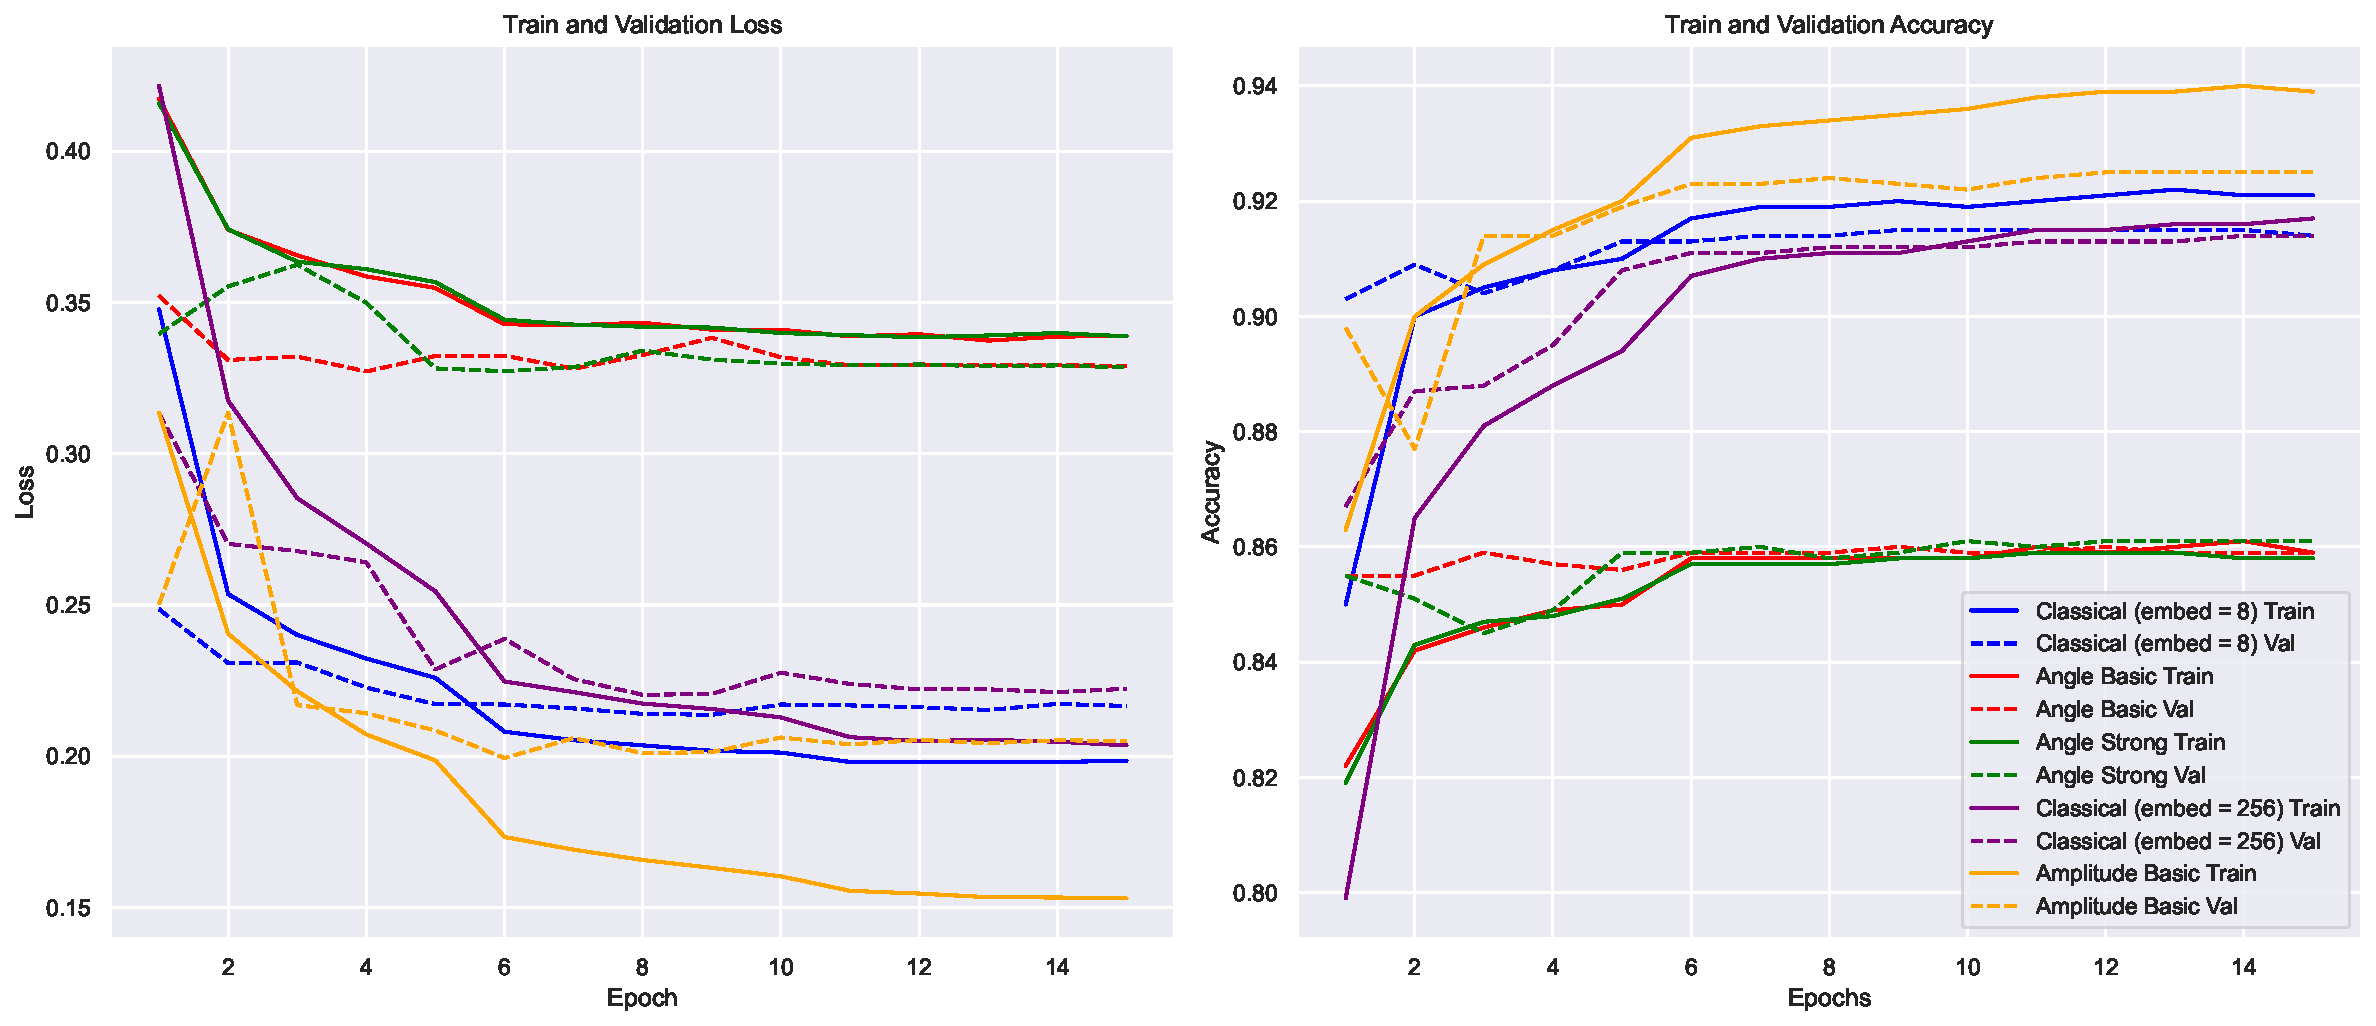
\includegraphics[width=0.98\textwidth]{img/plots/17_18_19_20_21.pdf}
    }
  \end{center}
  \vspace{-0.5cm}
  \caption{A loss plot and an accuracy plot for classical and quantum
    models on the Yelp dataset, using embedding sizes of 8 and 256,
    batch size of 64, trained for 20 epochs. The figures compare the
    classical transformer models to quantum models with angle encoding
    (3 layers of basic and strong \glspl{VQC}) and amplitude encoding
  (3 layers of basic \glspl{VQC}).}
  \label{fig:17_18_19_20_21}
\end{figure}

These plots in \autoref{fig:17_18_19_20_21} are largely consistent
with the previous results, with similar patterns emerging. Once
again, we observe early spikes in validation loss for both the strong
VQC (green) and amplitude encoding (yellow) models. This indicates
that these models are still struggling with initial instability
during training. Correspondingly, their accuracies also drop early on
before stabilising, reflecting the same training difficulties.

Despite this early volatility, both models recover and stabilise as
training progresses. The amplitude encoding model continues to
perform well, achieving the highest accuracy, while the strong VQC
remains comparable to other models, though it does not show any
significant advantage over the classical models or basic VQCs.

The superior performance of the amplitude encoding model suggests
potential improvements for future architectures. One idea is to
replace the angle encoding in the first transformer block layer with
amplitude encoding. By doing this, we can eliminate the encoding
layer that squeezes the input dimension from 768 to
\(2^8\) (256) and instead feed the entire input dimension of 768
directly into the quantum circuit using amplitude encoding. With 10
qubits, this could handle 1024 values, padding the input with zeros
if necessary to match the required size of 1024. In subsequent
layers, where the input dimension would be reduced to 10, angle
encoding could still be applied effectively.

Additionally, adding a Hadamard gate before the angle encoding in
these subsequent layers could increase the expressibility of the
quantum circuits~\cite{Sim_2019}. Moreover, replacing the CNOT
gates in the VQC with
parameterised controlled rotation gates would provide even greater
expressibility, potentially enhancing the ability of the model to capture
more complex relationships in the data~\cite{chu2022qmlp}. These
changes could help
address some of the initial instability observed in the current quantum models.

In summary, while the early fluctuations remain an issue, the overall
performance of the models aligns with previous findings. The
amplitude encoding model outperforms the others, and with further
optimisation, especially through architectural adjustments like those
mentioned above, the performance of quantum models could be improved
even further.

\subsection{Training Speed Comparison}
\label{subsec:training_speed_comparison}

\begin{table}[h]
  \caption{Training Time Comparison Across Deep Learning and Quantum
  Computing Frameworks.}
  \centering
  \begin{tabular}{|l|l|c|}
    \hline
    \textbf{Deep Learning Framework} & \textbf{Quantum Computing
    Framework}                       & \textbf{per Epoch}             \\ \hline
    PyTorch                          & PennyLane (CPU)
    & 4.5 hour                       \\ \hline
    PyTorch                          & PennyLane (CUDA)
    & 3.5 hour                       \\ \hline
    PyTorch                          & TensorCircuit (Tensorflow-CPU)
    & 2.5 hour                       \\ \hline
    PyTorch + Refactored Code        & PennyLane (CPU)
    & 10 min                         \\ \hline
    PyTorch + Refactored Code        & PennyLane (CUDA)
    & 7 min                          \\ \hline
    PyTorch + Refactored Code        & TensorCircuit (Tensorflow-CPU)
    & 3 min                          \\ \hline
    Tensorflow + Refactored Code     & TensorCircuit
    (Tensorflow-CUDA)                & \underline{2 min 45 sec}       \\ \hline
  \end{tabular}
  \label{tab:training_time_comparison}
\end{table}

In \autoref{tab:training_time_comparison}, we present a comparison of
training times across various deep learning and quantum computing
frameworks, as shown in the table. One of the key objectives of this
work was to significantly reduce training time, and we achieved this
goal by a considerable margin. Initially, using PyTorch combined with
PennyLane on the CPU took 4.5 hours per epoch, with CUDA providing a
slight improvement, bringing the time down to 3.5 hours. Switching to
TensorCircuit with TensorFlow on the CPU resulted in further
reductions, lowering the training time to 2.5 hours per epoch.

However, after refactoring the code to improve efficiency, the
training time saw dramatic improvements. With the refactored PyTorch
code running on PennyLane CPU backend, the training time was
reduced to just 10 minutes per epoch. Similarly, the CUDA version of
PennyLane with refactored code reduced the time to 7 minutes. The
most significant reduction came with TensorCircuit and TensorFlow on
both CPU and CUDA. The refactored code brought the training time down
to 3 minutes on TensorFlow-CPU, and using TensorFlow-CUDA, we
achieved the fastest training time of 2 minutes and 45 seconds per epoch.

It is important to note that the training time for the first epoch is
generally longer than for subsequent epochs due to \gls{JIT}
compilation in TensorCircuit. Once the compilation is complete, the
remaining epochs train much faster, further optimising the training process.

This dramatic reduction in training time highlights the effectiveness
of both code optimisation and leveraging more efficient quantum
computing frameworks like TensorCircuit. These improvements not only
make training quantum models more feasible but also align with our
objective of reducing the overall time required to train these models
significantly.
